\documentclass[conference]{IEEEtran}
\IEEEoverridecommandlockouts
\usepackage{cite}
\usepackage{amsmath,amssymb,amsfonts}
\usepackage{algorithmic}
\usepackage{graphicx}
\usepackage{textcomp}
\usepackage{xcolor}
\usepackage{bm} % Для \bm — жирный греческий и математические символы

\def\BibTeX{{\rm B\kern-.05em{\sc i\kern-.025em b}\kern-.08em
    T\kern-.1667em\lower.7ex\hbox{E}\kern-.125emX}}

\begin{document}

% Уравнения с исправленными обозначениями
\begin{equation}
\begin{cases}
    x_{1}^C = l_1 \cos{q_1} + l_2 \cos{q_2} + l_3 \cos(q_1 + q_2 + q_3), \\
    x_{2}^C = l_1 \sin{q_1} + l_2 \sin{q_2} + l_3 \sin(q_1 + q_2 + q_3);
\end{cases}
\label{eq:x1_and_x2_equations_1}
\end{equation}

\begin{equation}
    q_3 = -\frac{q_2}{2},
\label{eq:q2_and_q3_relation}
\end{equation}

\begin{equation}
\begin{cases}
    x_{1}^C = l_1 \cos{q_1} + l_2 \cos{q_2} + l_3 \cos\left(q_1 + \frac{q_2}{2}\right), \\
    x_{2}^C = l_1 \sin{q_1} + l_2 \sin{q_2} + l_3 \sin\left(q_1 + \frac{q_2}{2}\right);
\end{cases}
\label{eq:x1_and_x2_equations_2}
\end{equation}

\begin{equation}
\begin{cases}
    r = 2l_1 \cos\left(\frac{q_2}{2}\right) + l_3, \\
    \phi = q_1 - \frac{q_2}{2};
\end{cases}
\label{eq:r_phi}
\end{equation}

\begin{equation}
\begin{cases}
    q_1 = \phi + \arccos\left(\frac{r - l_3}{2l_1}\right), \\
    q_2 = 2 \arccos\left(\frac{r - l_3}{2l_1}\right); % Проверьте: возможно, опечатка в оригинале
\end{cases}
\label{eq:inverse_kinematics}
\end{equation}

% Уравнение движения: Q(t) → \mathbf{q}(t), \mathbf{Q}(t)
\begin{equation}
\mathbf{M}(\mathbf{q}) \ddot{\mathbf{q}} + \mathbf{C}(\mathbf{q}, \dot{\mathbf{q}}) \dot{\mathbf{q}} + \mathbf{K}(\mathbf{q}) = \mathbf{Q}(t),
\label{eq:motion}
\end{equation}

% Принцип Д’Аламбера: векторы — жирные
\begin{equation}
\sum_i \left( \mathbf{Q}_i - m_i \ddot{\mathbf{r}}_i \right) \cdot \delta \mathbf{r}_i = 0,
\label{eq:dynamics}
\end{equation}

% Уравнение Лагранжа: Q_i — скалярные компоненты
\begin{equation}
\frac{d}{dt} \left( \frac{\partial L}{\partial \dot{q}_i} \right) - \frac{\partial L}{\partial q_i} = Q_i, \quad L = T - \Pi
\label{eq:lagrange}
\end{equation}

% Wafer Robot
\begin{figure}[htbp]
    \centering
    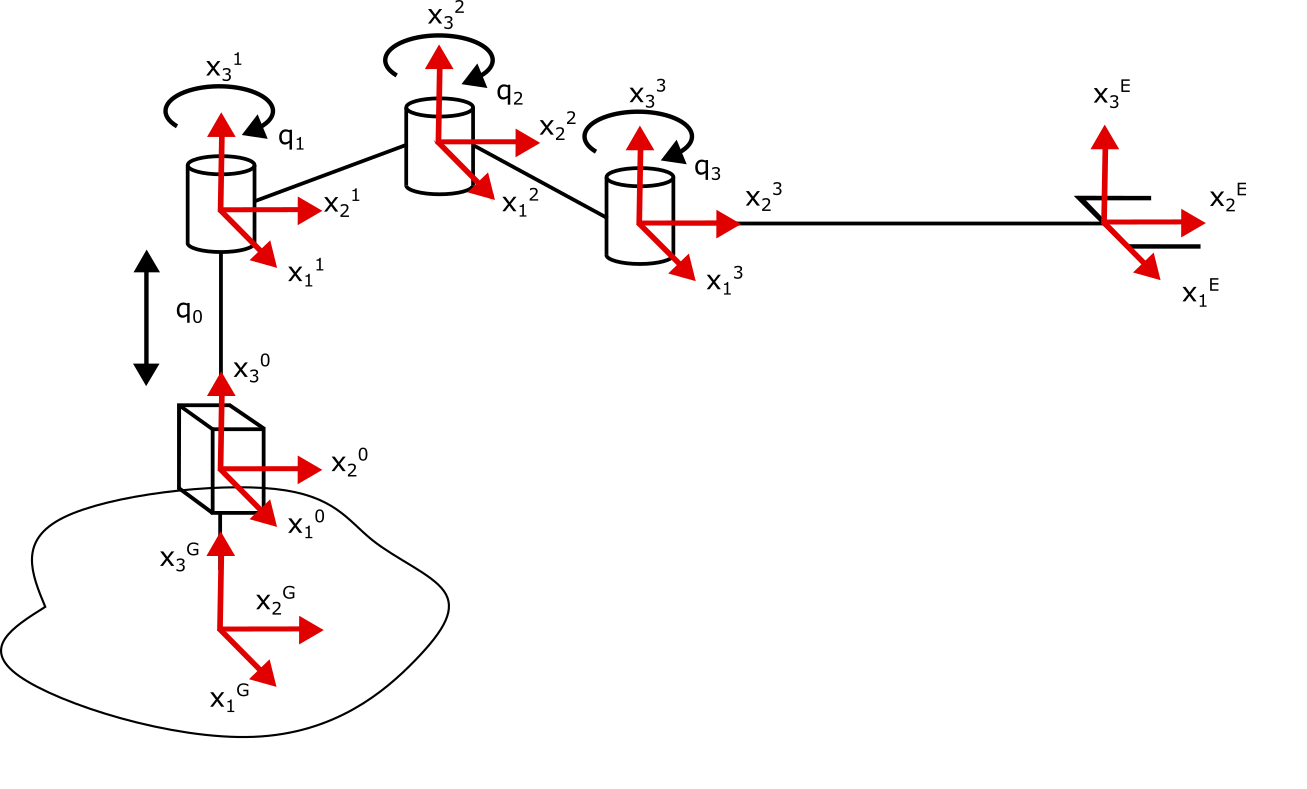
\includegraphics[width=\linewidth]{waffer robot.png}
    \caption{Kinematic scheme of robot.}
    \label{fig:wafer_robot}
\end{figure}

% Classic SCARA

\begin{figure}[htbp]
    \centering
    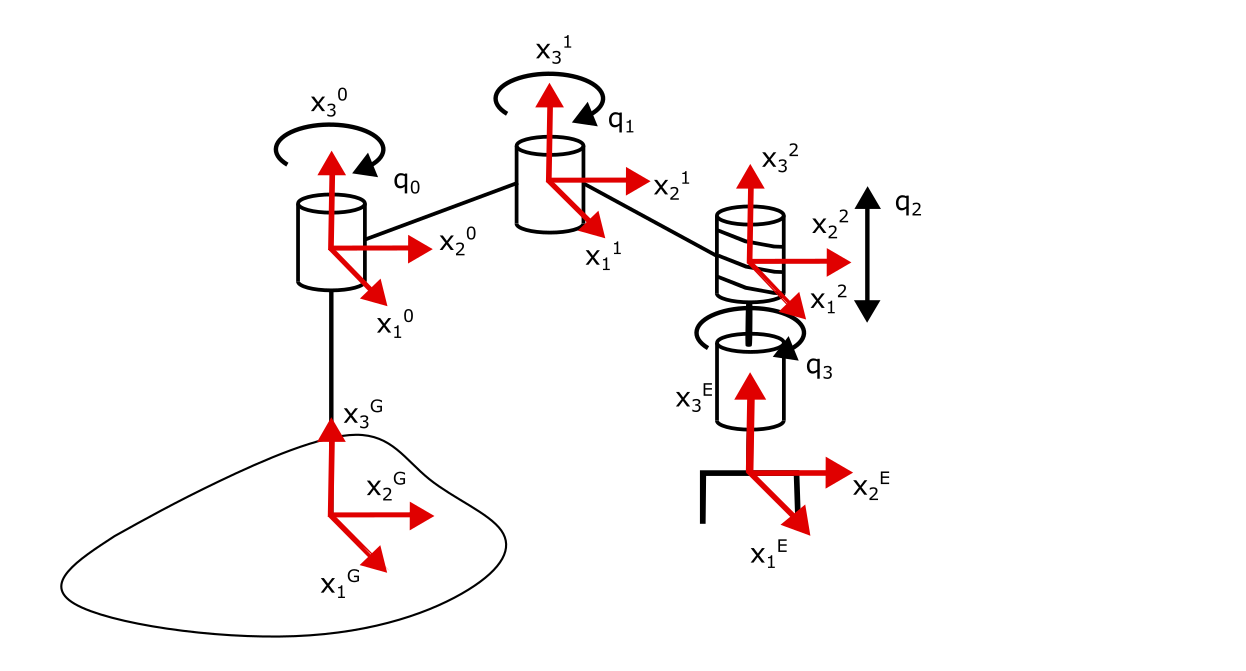
\includegraphics[width=\linewidth]{default scara.png}
    \caption{Classic SCARA robot kinematic scheme.}
    \label{fig:classic_scara}
\end{figure}

% Рисунок 3: Precise flex
\begin{figure}[htbp]
    \centering
    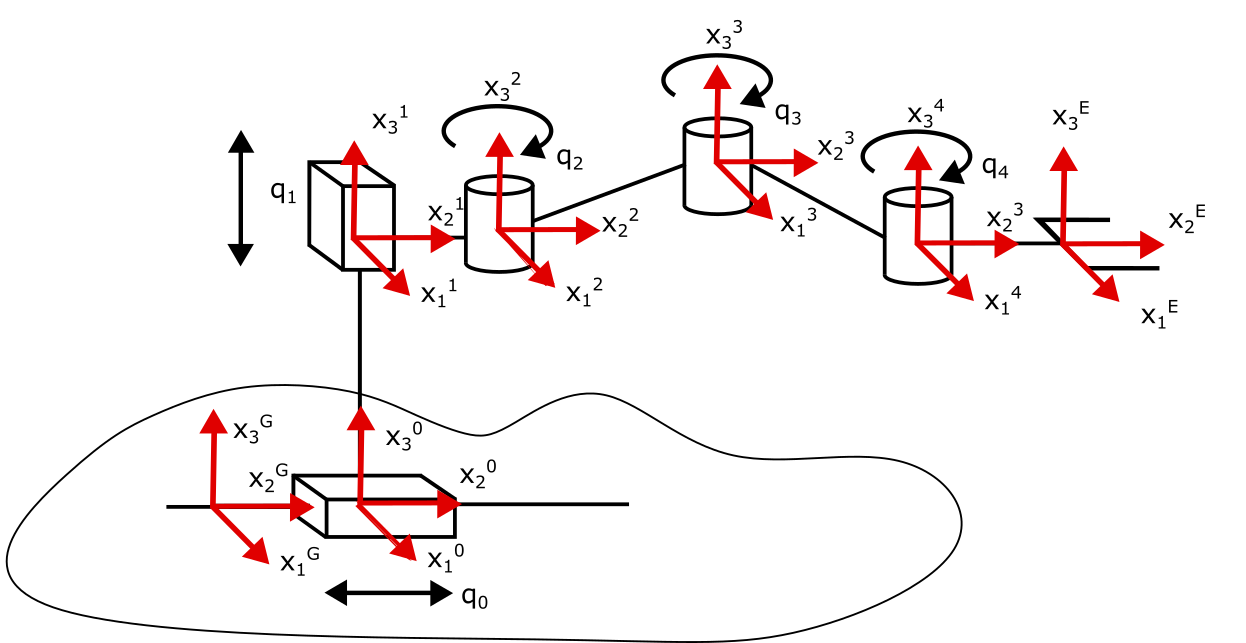
\includegraphics[width=\linewidth]{fancy scara.png}
    \caption{PreciseFlex 340 robot kinematic scheme.}
    \label{fig:modified_scara}
\end{figure}

% Рисунок 4: Sim window
\begin{figure}[htbp]
    \centering
    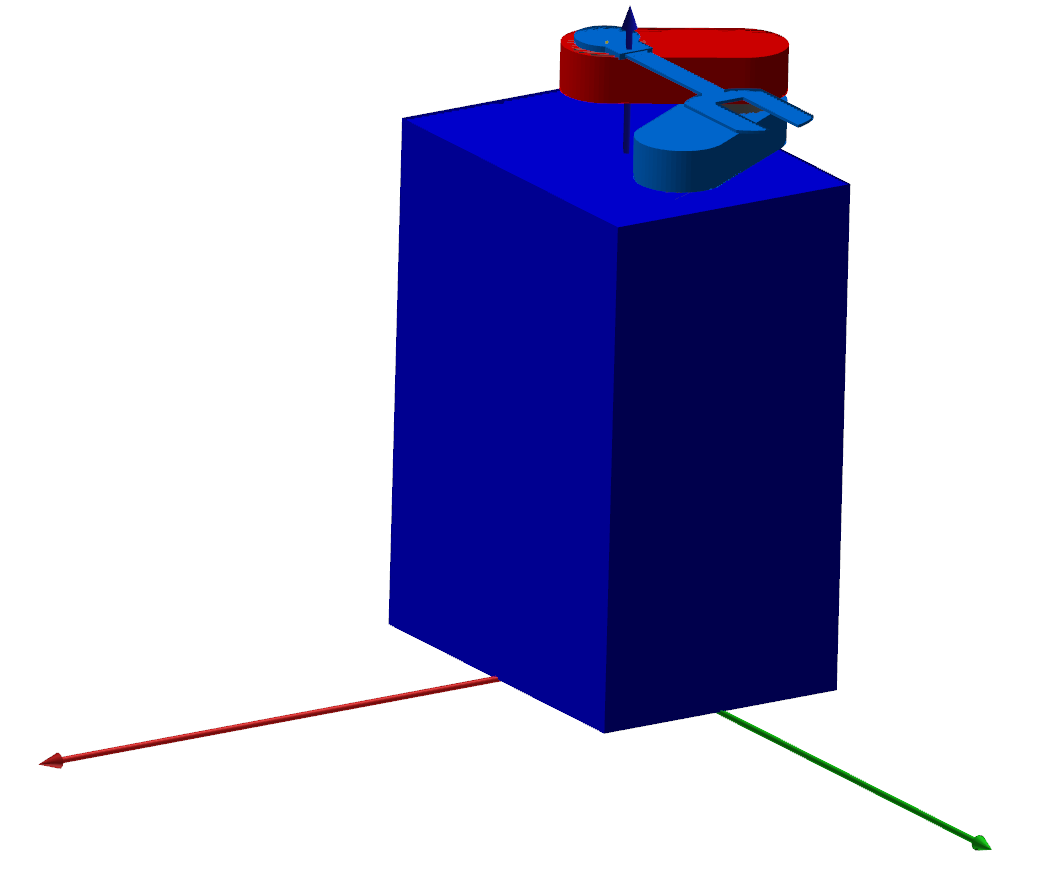
\includegraphics[width=\linewidth]{sim window.png}
    \caption{Exudyn simulation window view.}
    \label{fig:modified_scara}
\end{figure}

% Рисунок 5: Sim window
\begin{figure}[htbp]
    \centering
    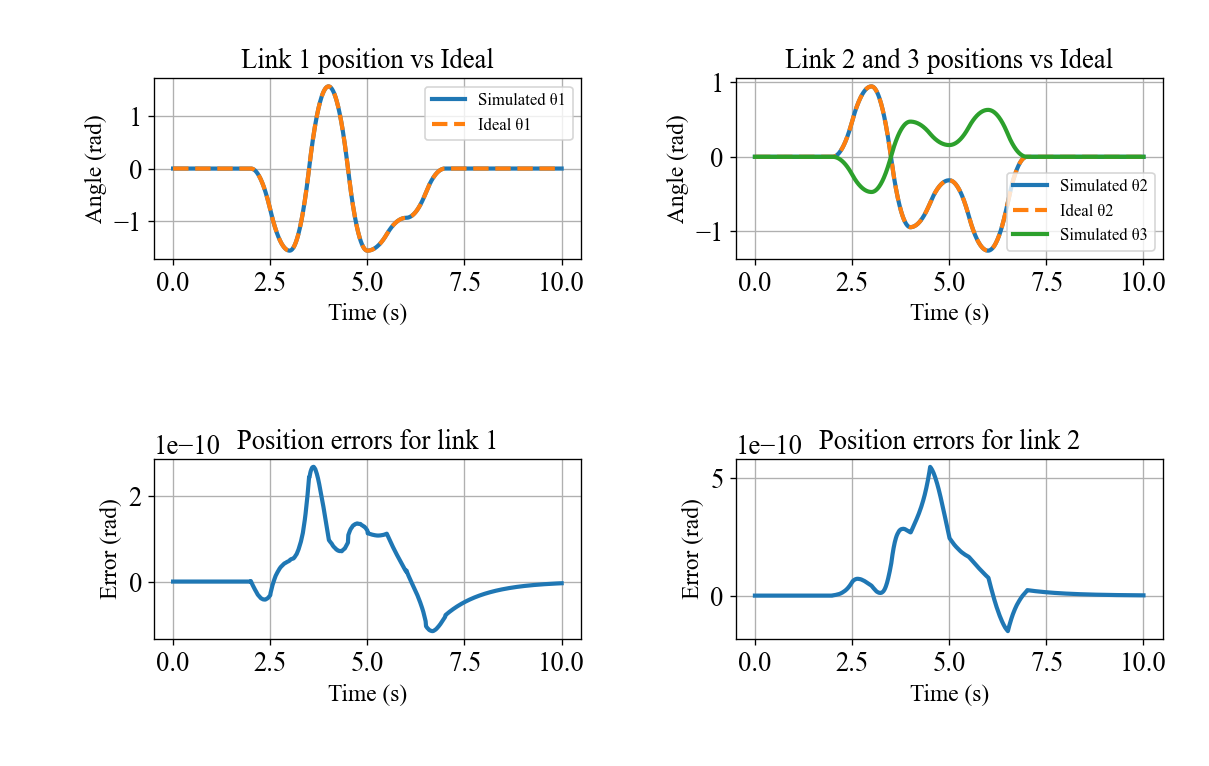
\includegraphics[width=\linewidth]{positions plot.png}
    \caption{Joint positions and position errors.}
    \label{fig:modified_scara}
\end{figure}


\end{document}